
%\vspace{-2mm}
\section{Introduction} \label{sec:intro}
%\vspace{-1mm}
Combinatorial optimization (CO), aiming to find out the optimal solution from discrete search space, has a pivotal position in scientific and engineering fields~\citep{papadimitriou1998combinatorial,crama1997combinatorial}. Most CO problems are NP-complete or NP-hard. Conventional heuristics or approximation requires insightful comprehension of the particular problem. Starting from the seminal work from \cite{hopfield1985neural}, researchers apply neural networks (NNs)~\citep{smith1999neural, vinyals2015pointer} to solve CO problems. The motivation is that NNs may learn heuristics through solving historical problems, which could be useful to solve similar problems in the future. %from the training data distribution. %\pan{Good, slightly revision needed for the last sentence} 

%Combinatorial optimization (CO), aiming to find out the optimal solution from discrete search space, has pivotal position in scientific and engineering fields~\citep{papadimitriou1998combinatorial,naseri2020application,crama1997combinatorial}. Most of the CO problems are NP-complete or NP-hard, conventional heuristics or approximation requires insightful comprehension of the particular problem's structure. By introducing machine learning for CO, ~\cite{hopfield1985neural} pique the researchers' interest in adopting neural networks~\citep{smith1999neural, vinyals2015pointer} to extract heuristics from the training data distribution. \pan{Good, slightly revision needed for the last sentence}
%In contrast, unsupervised LCO is superior in its faster training, good generalization, and strong
%capability of dealing with large-scale problems

Many NN-based methods~\citep{selsam2018learning,joshi2019efficient,hudson2021graph,gasse2019exact,khalil2016learning} require optimal solutions to the CO problem as supervision in training. However, optimal solutions are hard to get in practice and the obtained model often does not generalize well~\citep{yehuda2020s}. Methods based on reinforcement learning (RL)~\citep{mazyavkina2021reinforcement,bello2016neural,khalil2017learning,yolcu2019learning,chen2019learning,yao2019experimental,kwon2020pomo,kwon2021matrix,delarue2020reinforcement,nandwani2021neural} do not need labels while they often suffer from notoriously unstable training. Recently, unsupervised learning methods have attracted much attention~\citep{toenshoff2021graph,amizadeh2018learning,yao2019experimental,karalias2020erdos,wang2022unsupervised}. A common strategy of these methods is to design an NN whose output gives a solution to the CO problem and then train the NN via gradient descent by directly optimizing the CO objectives over a set of training instances. This strategy is superior in its faster training, good generalization, and strong capability of dealing with large-scale problems. % which therefore have attacted attention in many recent studies~\citep{toenshoff2021graph,amizadeh2018learning,yao2019experimental,schuetz2022combinatorial,karalias2020erdos,wang2022unsupervised}. %Among them, \cite{karalias2020erdos} proposed EGN with performance guarantee , which has recently got generalized by~\cite{wang2022unsupervised} to design proxy via the `entry-wise concave' relaxation-and-rounding principle for the performance guarantee.  and then train the NN with gradient descent which directly optimizes the CO objective

Despite the prominent progress, current unsupervised learning methods always optimize NNs towards an \emph{averaged good} performance over training instances. This means even if a testing instance comes from the same distribution of the training instances, the solution to this single instance may not have good quality, let alone the case when the testing instance is out-of-distribution (OOD). This induces a concern when we apply NNs in practice because practical problems often expect to have a good solution to every encountered instance. For example, allocating surveillance cameras is crucial for each-time exhibition in every art gallery. Solvers when applied to this problem~\citep{o1987art,yabuta2008optimum} should output a good solution every time. Traditional CO solvers are designed toward this goal. However, it is time-consuming and unable to learn heuristics from historical instances. So, can we leverage the benefit of learning from history with the goal of achieving an instance-wise good solution instead of an averaged good solution?

This motivates us to study a new formulation of unsupervised learning for CO. We regard the objective of learning from history as to search for a good initialization for each future instance rather than give a direct solution. Since in practice, future instances are unavailable during the training stage, we propose to view each training instance as a pseudo-new instance for the rest training instances. 
Then, our learning objective is to learn a good initialization of this model, such that further optimization of the initialization could achieve good solutions on each of these pseudo-new instances. We observe meta learning is suitable to implement this idea and propose to adopt MAML~\citep{finn2017model} in our training pipeline as a proof of concept. Note that the step of optimization on each pseudo-new instance shares a similar spirit with fine-tuning a model over each down-streaming task as traditional meta learning does. However, each task in our case corresponds to optimization over each training instance. 

We name our method \proj by extending the previous framework EGN~\citep{karalias2020erdos} via meta learning. Our key observation is that with this new objective, even the initial solution given by \proj (before fine-tuning on a test instance) is substantially better than the solution given by EGN and other methods that optimize the averaged performance over training instances. Our conjectured reason is that the new objective, by taking into account fine-tuning the model over new instances, trains the model to avoid being trapped into a local minimum induced by each training instance while being more adaptive to the changes of optimization landscapes across instances.%distinguish valleys with good local minima in the optimization landscape for each instance from those with bad local minima. The model may directly put initial solutions into those good valleys.             



% objective of training the NN over historical instances as to search a good initialization for each future instance rather than give a direct solution. The NN is allowed being further optimized over each new instance. As in practice the distribution of future instances is unavailable during the training stage, we view each training instance as a new instance. The latter per-instance optimization shares a similar spirit as fine-tuning a RL model, while our key observation is that with this new objective, even just the initialization given by the NN (before fine-tuning) is substantially better than the solution given by optimizing the averaged CO objectives over training instances. Our conjectured reason is that the new objective takes into account the dynamics of fine-tuning the model over new instances, which helps the model distinguish valleys with good local minima from those with bad local minima in the optimization landscape, and directly put initial solutions into good valleys.             

% The new objective can be optimized via the meta-learning pipeline. 


% Most unsupervised learning methods follow a common strategy. Given a class of CO problems, say minimum vertex cover (MVC), they design an NN that takes the graph as input and outputs a solution to the MVC problem over this graph. To learn some valid heuristics, the NN has to be exposed to a set of graphs that often follow a distribution, and use MVC as the training objectives on these graphs. The obtained NN is expected to give a good MVC solution over a new graph that follows the same distribution. However, this is a really ideal setting, because in practice, it is hard to guarantee that the new graph comes from the same distribution. Even if this is true, the above framework may only guarantee an averaged performance over the distribution, while practical problems always expect to have a good solution to every encountered instance. Think about using the learned MVC solver to dynamically allocate  erw

%the actual goal of CO is to find the optimal solution for each single instance encountered in the testing stage. For instance, the art gallery~\citep{o1987art,yabuta2008optimum} problem is a real-world application of the minimum vertex covering problem, which asks to use as few surveillance cameras as possible to cover all the passages of the entire exhibition venue. In such problem, people only have one single venue to optimize, instead of considering the average solution performance for many venues. An intuitive idea to solve for the single instance optimality is to directly run traditional CO solvers or train networks on the instance, which is time-consuming and unable to use the heuristics from the historical data. Therefore, our main idea is motivated by training the networks so as to not only make use of the heuristics learnt from historical graphs but also pursue the optimality for each single testing instance instead of the optimality over expectation. We lend ourselves to a special formulation of machine learning, meta-learning specifically~\citep{finn2017model,rajeswaran2019meta,nichol2018first}. We use the historical graphs to obtain a good initialization of the network parameters such that a limited-step (one-step in our case for comparable time-efficiency) fine-tune could make a leap towards the per-instance optimality~\citep{finn2017model}. In addition, instances in CO could be more distinct with each other, making themselves to be independent tasks rather than as strongly connected with others as in common ML-based problems, which is naturally similar with the `zero-shot learning' setting. Aligned with the distinct characteristic of CO instances, introducing meta learning to the unsupervised learning for CO framework could not only boost the models' performance but also improve the generalization ability.





%the graph is indeed generated from the same    


%and then train the NN with gradient descent which directly optimizes the CO objective

%The NN is exposed to a set of training examples  


%To capture the heuristics behind the problem, they often 
%Despite the prominent progress, most of the works led by EGN target to achieve high performance in the expectation sense over a certain data distribution. Note that the actual goal of CO is to find the optimal solution for each single instance encountered in the testing stage. For instance, the art gallery~\citep{o1987art,yabuta2008optimum} problem is a real-world application of the minimum vertex covering problem, which asks to use as few surveillance cameras as possible to cover all the passages of the entire exhibition venue. In such problem, people only have one single venue to optimize, instead of considering the average solution performance for many venues. An intuitive idea to solve for the single instance optimality is to directly run traditional CO solvers or train networks on the instance, which is time-consuming and unable to use the heuristics from the historical data. Therefore, our main idea is motivated by training the networks so as to not only make use of the heuristics learnt from historical graphs but also pursue the optimality for each single testing instance instead of the optimality over expectation. We lend ourselves to a special formulation of machine learning, meta-learning specifically~\citep{finn2017model,rajeswaran2019meta,nichol2018first}. We use the historical graphs to obtain a good initialization of the network parameters such that a limited-step (one-step in our case for comparable time-efficiency) fine-tune could make a leap towards the per-instance optimality~\citep{finn2017model}. In addition, instances in CO could be more distinct with each other, making themselves to be independent tasks rather than as strongly connected with others as in common ML-based problems, which is naturally similar with the `zero-shot learning' setting. Aligned with the distinct characteristic of CO instances, introducing meta learning to the unsupervised learning for CO framework could not only boost the models' performance but also improve the generalization ability.

\begin{figure}[t]
%\vspace{-1.2cm}
    % \centering
     %\begin{subfigure}[c]{0.32\textwidth}
         \centering
         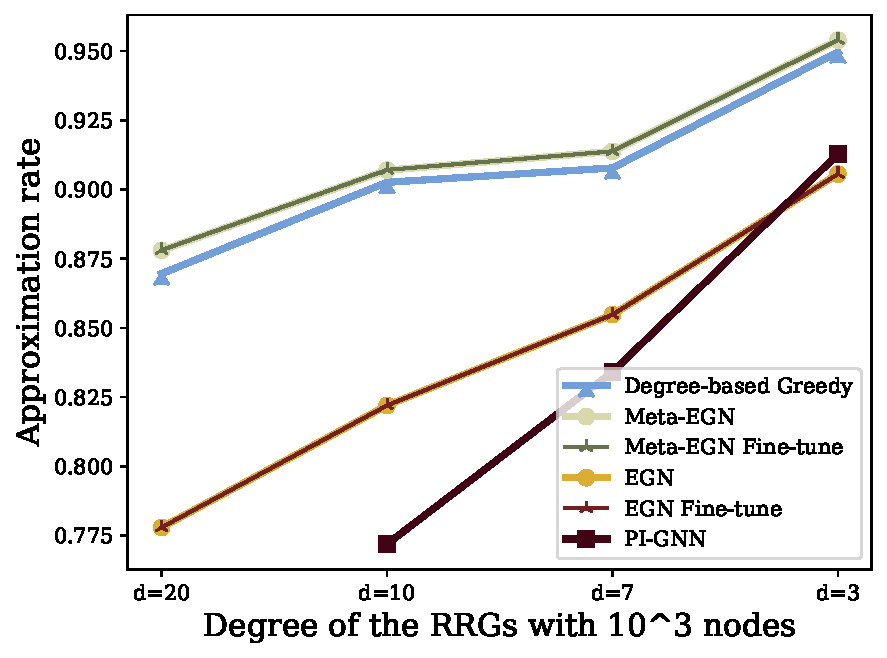
\includegraphics[width=0.32\textwidth]{iclr2023/img/intro/mis_10_3.pdf}
%         \vspace{-0.6cm}
      %   \caption{Performance with $10^3$ vertices}
       %  \label{fig:mis_103}
     %\end{subfigure}
     \hfill
     %\begin{subfigure}[c]{0.32\textwidth}
      %   \centering
         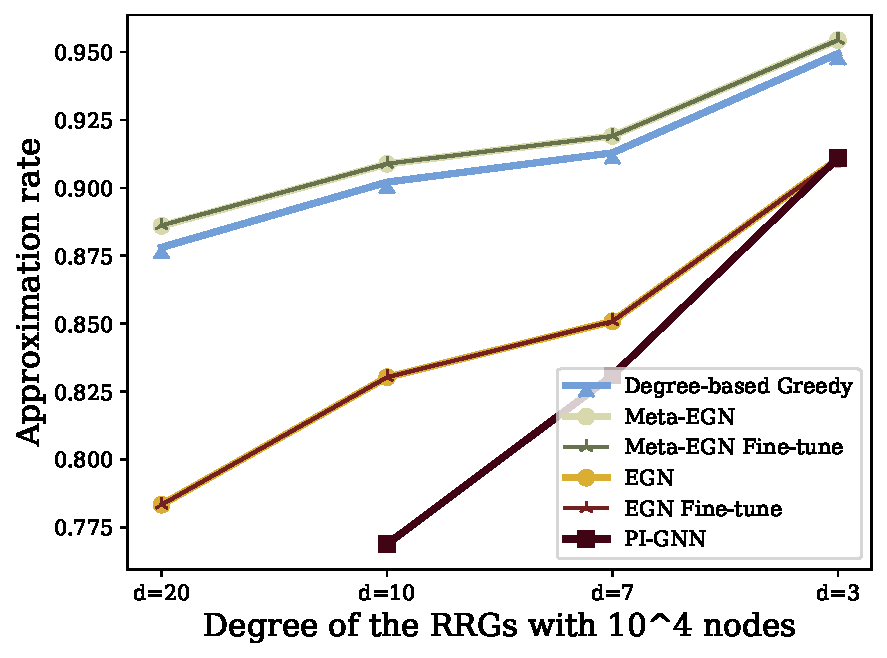
\includegraphics[width=0.32\textwidth]{iclr2023/img/intro/mis_10_4.pdf}
       %  \vspace{-0.6cm}
        % \caption{Performance with $10^4$ vertices}
        % \label{fig:mis_103}
     %\end{subfigure}
     \hfill
     %\begin{subfigure}[c]{0.32\textwidth}
      %   \centering
         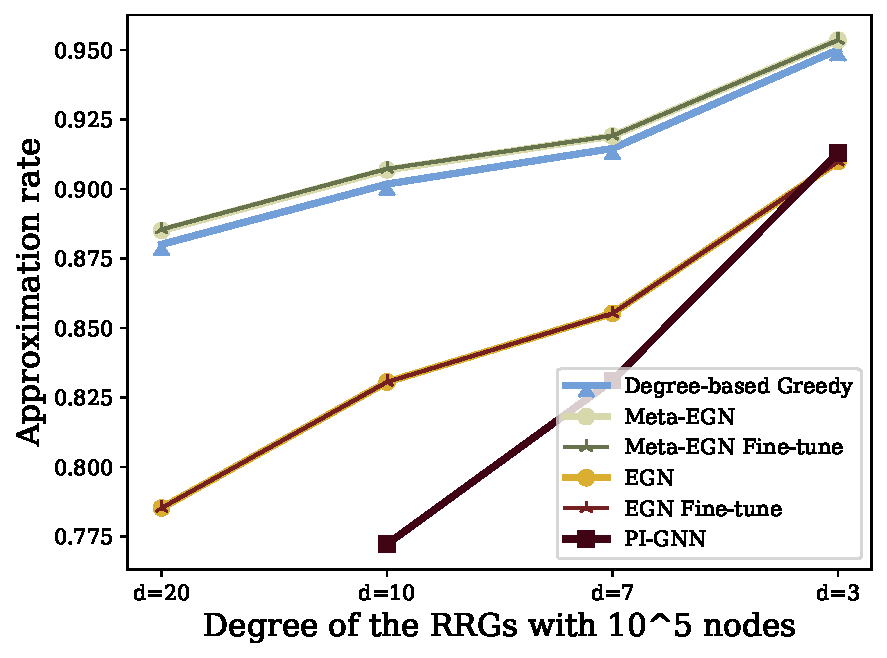
\includegraphics[width=0.32\textwidth]{iclr2023/img/intro/mis_10_5.pdf}
       %  \vspace{-0.6cm}
        % \caption{Performance with $10^5$ vertices}
         %\label{fig:mis_103}
    % \end{subfigure}
     \vspace{-0.3cm}
        \caption{Approximation Rates of different methods in the MIS problem.  \proj and EGN~\citep{karalias2020erdos} are trained on RRGs with $1000$ nodes and with node degree randomly sampled from $3,7,10,20$. \proj and EGN are evaluated over larger RRGs with $10^3\sim10^5$ nodes. More details about the setting are in Secs.~\ref{sec:settings} and~\ref{sec:MIS}. Meta-EGN outperforms DGA~\citep{angelini2019monte} by about $0.3\%-0.5\%$ in approximation rates on average.}
        \label{fig:mis}
        \vspace{-0.6cm}
        
\end{figure}

%instead of the per-instance optimality \pan{I think this statement is too technical.}. Note that the actual goal of CO is to find the optimal solution for each single instance encountered in the testing stage. There always exists a performance gap between the current optimization goal and the actual goal of CO, unless the model could learn an almost `one-to-one' mapping from the exponential input space to every optimal solution, which is currently impractical due to the limitation on the model's expressive power~\cite{chen2019learning,srinivasan2019equivalence,you2019position}, the training data volume~\citep{yehuda2020s} and the number of parameters \pan{This is so technical. Also, the previous references on expressive power are incorrect. The better way is to use practical example to claim in practice one-example instance is what is needed. Claim that generalization is importance.}. This gap seems passable in other ML applications such as computer vision or natural language  \pan{No one can understand this... This type of discussion should be put into the methodology part and pair it with an illustrative figure.}. These problems have less non-convex optimization landscapes, where different non-trivial local minima share similar values that are close to the global optimum~\citep{choromanska2015loss,kawaguchi2019every} \pan{Have you checked these references?}, which enables the networks to easily find out one in the expectation sense. Also, due to the regular and well-clustered feature map, once a good local optimum over expectation is achieved, the networks could easily grasp mapping patterns for interpolations on unseen data to obtain acceptable per-instance performance \pan{Do we need to claim per-instance performance of non-CO tasks? Per-instance performance cannot be pursued is because of objective is un-defined when without labels}. But as to CO, such gap could be significantly magnified. It's more difficult for CO problems to reach even the optimum over expectation. The non-convex optimization landscape of CO is intricate with high variance \pan{references?}, trapping the models in the non-trivial local optima without anymore guarantees on the distance from the global optimum \pan{Kind of over-claim because in traditional non-CO tasks, there is also no guarantee, also needed to be put into Method part}.  Also, interpolation on unseen data could be more easily spoiled \pan{interpolation?}. Instances in CO are more distinct from each other \pan{These descriptions are so subjective}, `similar' inputs with slight difference (i.e. adding/removing a single edge or vertex) might lead to entirely different solutions \pan{do you mean different optimal solutions? Can it be still a good approximate solution? Why I need optimal solution? Traditional ERM also does not guarantee optimal solution. The statement should be rephrased}. More aptly, each instance in CO appears to be an independent `task' rather than being as strongly connected with others as in common ML-based problems, which is naturally similar with the `few-shot learning' or even `zero-shot learning' setting \pan{This is not strong/certain enough. It is zero-shot learning problem. Also, the connection to zero shot should be proposed after the next paragraph.}.

%Thanks to unsupervised learning which makes gradient based fine-tuning on testing data a reality, An intuitive idea to curtail the gap is to train the objective on single instances. However, directly solving the per-instance optimality from scratch would not only be even more easier to trap the parameters into trivial local optima but also be less time-efficient \pan{Why?} than other CO solvers \pan{Do you assume the former is NN-based when saying this?}. To address the issues, we lend ourselves to a special formulation of machine learning, meta-learning specifically. We use the historical graphs to obtain a good initialization of the network parameters such that a limited-step (one-step in our case for comparable time-efficiency) fine-tune could make a leap towards the per-instance optimality \pan{Do you need to cite MAML?}. Also, aligned with the distinct characteristic of CO instances by regarding them as independent tasks, the meta method naturally ameliorates the models' generalization ability in the case, as displayed in Figure~\ref{intro:learning_curve} \pan{This figure does not show generalization. }. \pan{Two aspects of the benefits should be emphasized: Per-instance optimality \& generalization. I do not think these two aspects are properly explained and motivated.}

We demonstrate the benefits of \proj via experiments within three benchmark CO problems (max clique, vertex cover, and max independent set) on multiple synthetic graphs and three real-world graph datasets, with the number of nodes ranging from $100$ to $5000$. \proj significantly outperforms state-of-the-art learning-based baselines~\citep{karalias2020erdos,toenshoff2021graph}, greedy algorithms, and the commercial CO solver Gurobi9.5~\citep{Gurobi} in most cases. \proj also shows super OOD generalization performance when the training and test datasets are different or have graphs of entirely different sizes.   %significantly outperforms We also compare different methods over OOD graphs?}

%brought by our method in all the tasks over all the datasets, our framework also outperforms the previous state-of-the-art unsupervised frameworks~\citep{toenshoff2021graph} and the greedy algorithms. Our method also exceeds the current state-of-the-art commercial CO solver Gurobi9.5~\citep{Gurobi}, especially in large scale and hard instances. We do extensive experiments across the graph distribution (real-to-real, real-to-synthetic, synthetic-to-real, synthetic-to-complement) and across scales (from $500$ to $2000$) to further confirm our conjecture on our meta objective's ability in improving the generalization ability. Surprisingly, we also find our method could outperform the EGN even without the one-step fine-tuning, we attribute the phenomenon to meta's ability in finding out better local minima as initialization.


%We observe a significant boost in performance on EGN~\citep{karalias2020erdos} brought by our method in all the tasks over all the datasets, our framework also outperforms the previous state-of-the-art unsupervised frameworks~\citep{toenshoff2021graph} and the greedy algorithms. Our method also exceeds the current state-of-the-art commercial CO solver Gurobi9.5~\citep{Gurobi}, especially in large scale and hard instances. We do extensive experiments across the graph distribution (real-to-real, real-to-synthetic, synthetic-to-real, synthetic-to-complement) and across scales (from $500$ to $2000$) to further confirm our conjecture on our meta objective's ability in improving the generalization ability. Surprisingly, we also find our method could outperform the EGN even without the one-step fine-tuning, we attribute the phenomenon to meta's ability in finding out better local minima as initialization.

Moreover, recently, \cite{angelini2022cracking} have shown that the learning-based method in~\citep{schuetz2022combinatorial} could not achieve comparable results with the degree-based greedy algorithm (DGA)~\citep{angelini2019monte} in the max independent set (MIS) problem on large-scaled random-regular graphs (RRGs), which raises attentions from machine learning community. We observe the issues come from two aspects: (1) graph neural networks (GNNs) used to encode the regular graph suffer from the node ambiguity issue due to their limited expressive power~\citep{xu2018powerful}; (2) the model in~\citep{schuetz2022combinatorial} did not learn from history but was directly optimized over each testing case, which tends to be trapped into a local optimum. By addressing these two issues, \proj can consistently outperform DGA while maintaining the same time complexity to generate solutions. Fig.~\ref{fig:mis} show the results. %Meta-EGN and EGN are only trained on graphs with $10^3$ nodes and test on graphs with $10^3\sim10^5$ nodes.

%that our meta learning framework for CO could indeed learn heuristics from the greedy algorithms, which could achieve better performance, maintain the same time complexity and obtain good generalization ability across very large scales changes from $10^2$ to $10^5$, even before the fine-tuning step on testing data. The performance of our framework is shown in Figure~\ref{method:learning_curve}\hl{to be revised}.

%posed a big concern for ML for CO by

\iffalse
In addition, parameters of the models tend to be more conservative due to the `penalty' constraint in the training objective. Considering the penalty, a tiny change (i.e. setting one optimization variable from 0 to 1) on prediction might directly ruin the loss value. Thus rather than obtaining insignificant reward for better approximations for certain instances by taking the risk of breaking any constraint among the training data, the parameters prefer to guarantee feasible but not the best solution that it could reach for the whole data distribution, which would further widen the gap.


$\bullet$ Recent years have witnessed a boost in machine learning for combinatorial optimization. 
\pan{General motivation on learning for CO should be provided.}

formulation of problem (The goal of CO, in words not formulation), 
\begin{align*}
    \min_{X\in \Omega} f(X;D).
\end{align*}
introduce what methods could solve the problem (supervised in 1-2 sentences).

\pan{Do we need to slightly explain why we consider unsupervised learning?}
$\bullet$ Among the outstanding works, the Erd\H{o}s goes neural (EGN) introduces an unsupervised learning framework guided by the probabilistic methods. 

\pan{The following paragraph is too technical for intro. I suggest you first write Sec. 3 to make sure your notations/terminology are all comfortable in your mind. Then, write Sec. 1. Then, revise Sec. 3 according to Sec. 1. I still think there is some very basic intuition to motivate our formulation, which you do not need to directly intro ERM formulation.} \pan{For example ``Our idea comes from the simple first principle of the standard CO formulation: The goal of CO is to find the optimal solution for every instance encountered in the testing stage. However, previous works on unsupervised learning for CO \cite{EGN and others} always adopts an learning objective whose goal is to achieve optimality in the expectation sense over a certain distribution of instance, instead of optimality per instance, which yields suboptimal performance.''}\pan{Raise one/two real-world example.} But EGN formulates the training goal of the unsupervised learning for CO in an empirical risk minimization (ERM) form:  Suppose there a data distribution $D\sim P_{D}$ \pan{$\mathbb{P}_D$}. EGN aims to learn a parameterized randomized algorithm $P(X|D,\theta)$ to generate $X\in \Omega$ so as to minimize $E_{D\sim P_D}E_{X\sim P(X|D,\theta)}(f(X;D))$  \pan{$\mathbb{E}_D$}. That is
\begin{align*}
    \min_{\theta}E_{D\sim P_D}E_{X\sim P(X|D,\theta)}(f(X;D)).
\end{align*}
This goal aims for a good performance under the expectation considering the distribution of the testing dataset.

\pan{Define}
\begin{align*}
    l(\theta, D):\triangleq \mathbb{E}_{X\sim \mathcal{A}_{\theta}(D)}[f(X;D)] 
\end{align*}

\begin{align*}
     \textbf{Prev. Goal:} \min_{\theta}\mathbb{E}_D[l(\theta, D)]
\end{align*}

Actually, the goal is to do $\min_{\theta} l(\theta, D)$ for any $D\in \mathbb{P}_D$. 


\pan{However, directly solving $\min_{\theta} l(\theta, D)$ suffers from two issues 1) could easily be trapped into local OPT; (Cite non-convex landspace paper and claim the tendency to be in bad local optimal) 2) Take a lot of time to optimize. To address both issues, we lend ourselves to a special formulation of machine learning, meta learning specifically. We use the historical graphs to obtain a good initialization of $\theta$ such that a limited-step (one-step in our case) finetune of $\theta$ may make it good for each instance.}

%So, we propose .... Learning here essentially works for getting a good initialization for the downstream instance-wise optimization. We expect the initialization to be already very good. A limited-step (one-step in our case) finetune may make it even better.}

\pan{Define}
\begin{align*}
    \tilde{l}(\theta, D):\triangleq \mathbb{E}_{X\sim \mathcal{A}_{\theta_D}(D)}[f(X;D)], s.t., \theta_D=\theta - \nabla_{\theta} l(\theta, D) 
\end{align*}

\pan{Our goal:}
\begin{align*}
    \rightarrow \textbf{Our Goal:}\;\min_{\theta}\mathbb{E}_D[\tilde{l}(\theta, D)] 
\end{align*}


\pan{Define}
\begin{align*}
    \tilde{l}(\theta, D): \mathbb{E}_{X\sim \mathcal{A}_{\theta_D^*}(D)}[f(X;D)], s.t., \theta_D^*= \argmin \mathbb{E}_{X\sim \mathcal{A}_{\theta}(D)}[f(X;D)]\;\text{initialized by $\theta$}
\end{align*}

\pan{Our goal:}
\begin{align*}
    \rightarrow \textbf{Our Goal:}\;\min_{\theta}\mathbb{E}_D[\tilde{l}(\theta, D)] 
\end{align*}

% \pan{Define}
% \begin{align*}
%     \tilde{l}(\theta, D):\triangleq \mathbb{E}_{X\sim \mathcal{A}_{\theta-\nabla l(\theta, D) }(D)}[f(X;D)] \;\text{with initialization $\theta= \theta^{(0)}$}
% \end{align*}


% \begin{align*}
%     \textbf{Our Training:} \frac{1}{n}\sum_{i=1}^n \min_{\theta_i} l(\theta_i, \theta_i^{(0)}, D_i)
%     \,\text{where} \,\theta_i^{(0)} = \argmin_{\theta}  \frac{1}{n}\sum_{j=1,j\neq i}^n l(\theta, D_j) \\
%     \rightarrow \textbf{Our Goal:}\;\mathbb{E}_D[\min_{\theta}l(\theta, \theta^{(0)}, D)] ,\text{where} \,\theta^{(0)} = \argmin_{\theta}  \mathbb{E}_D[l(\theta, D_j)] \\
% \end{align*}
$\bullet$ 
Nevertheless, for CO problems, instead of aiming to get an expected minimized objective value on the whole testing set, a more reasonable goal is to achieve as high performance as possible on each single testing instance, which could be written as follows: 

\begin{align*}
   E_{D\sim P_D}  \min_{\theta} E_{X\sim P(X|D,\theta)}(f(X;D)).
\end{align*}

Also, in many difficult CO problems, The optimal solution to very similar configurations may be entirely different, which makes it very hard to find the pattern.
(Here we might take zero-shot learning problem for comparison).

To fulfill the goal above and formulate the problem in a more reasonable manner, we aim to learn a network to give a good initialization for CO problem, then on each testing instance, we fine-tune the initialization produced by the NN for better performance given a time budget which is comparable to the current prevailing methods. This naturally corresponds to the idea of meta-learning, which targets at training the fine-tuning potential of the model to achieve better performance after several further gradient steps on each testing instance, making it much closer to our goal.

\pan{Here, first claim the theoretical benefits: 1). Performance. 2) Generalization. Then say experiments verify such. Use one paragraph to say nature paper v.s. nature paper comments (large scale, time efficient).}

\pan{To the best of our knowledge, we are to first...}

$\bullet$ Experiment results have shown the great potential that meta could bring to EGN from the following aspects: 1) highly boosts in performance (one real task and synthetic based on RB model), outperforms the SOTA CO solver Gurobi9.5 in hard tasks 2) even better generalization ability between the real datasets and the synthetic datasets 3) guided by simple baselines, has the potential to outperform the simple baselines (MD-GA).
\fi